\chapter{Implementation}

% \epigraph{The best presents don't come in boxes.}{Bill Watterson}


\begin{figure}[H]
	\centering
	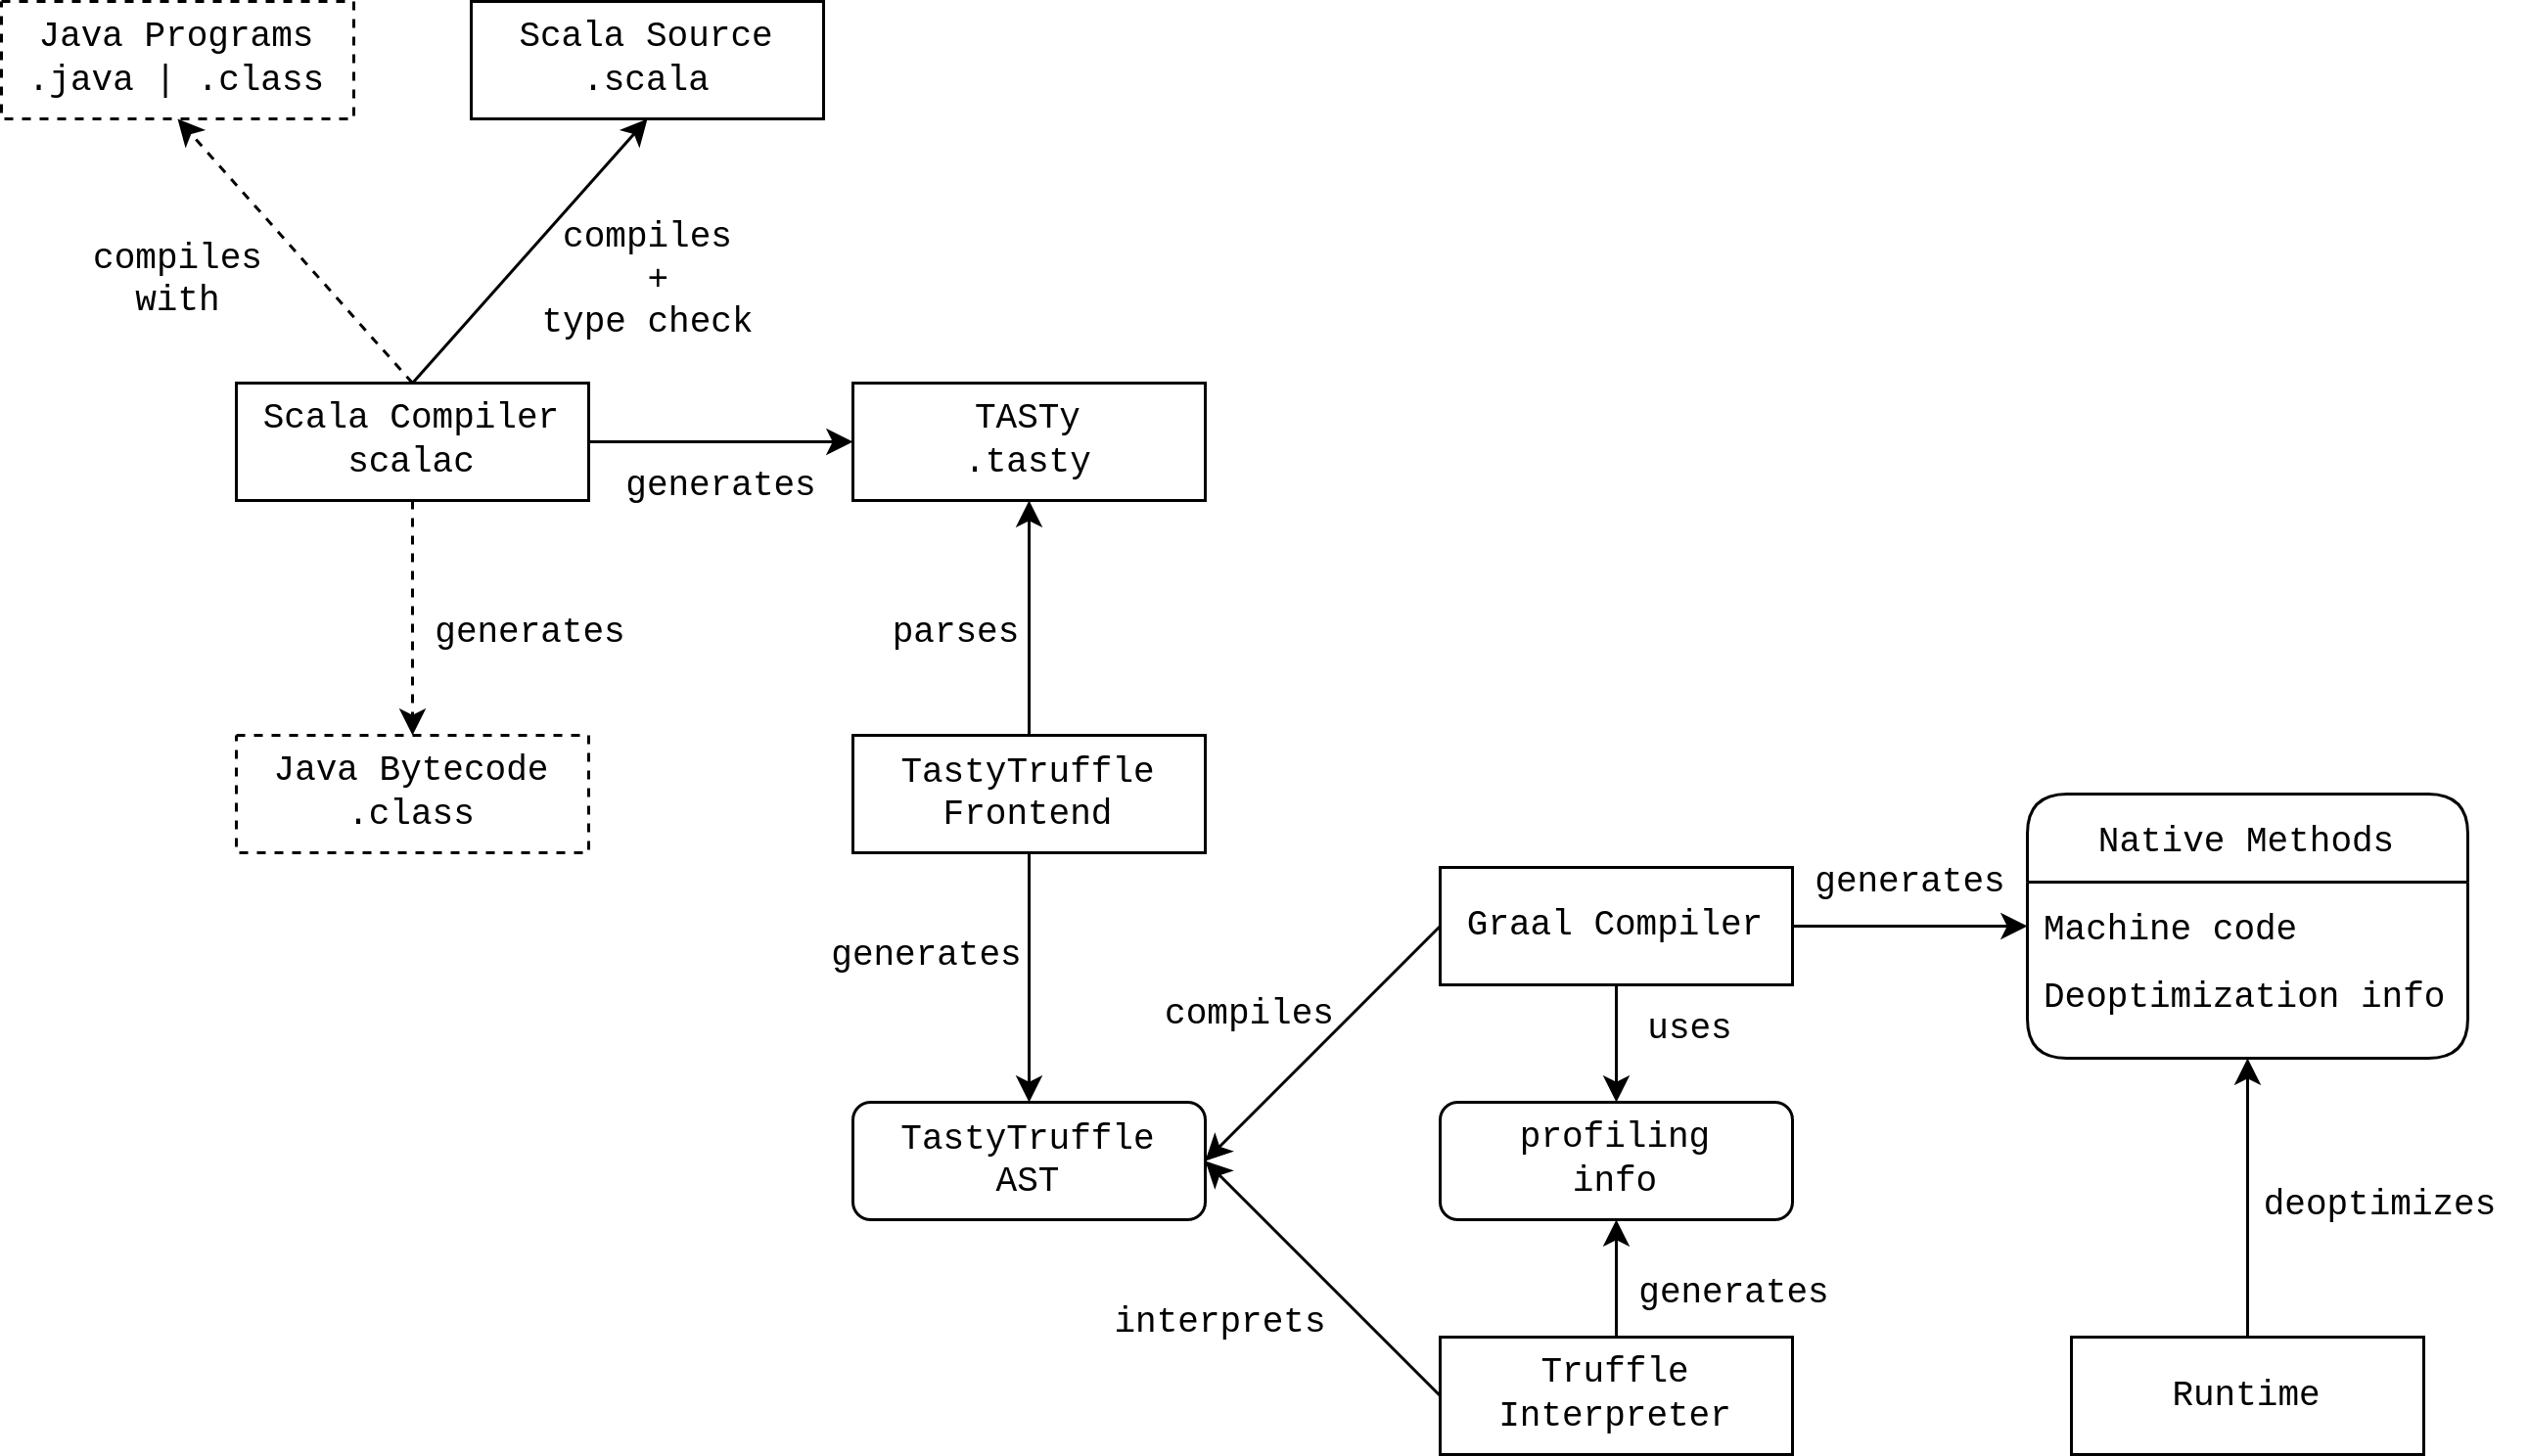
\includegraphics[width=0.5\textwidth]{figures/tastytruffle-pipeline.png}
	\caption{TastyTruffle in the context of the Scala compilation pipeline.}
\end{figure}

\section{Case Study: A List in TastyTruffle}

\begin{figure}[H]
	\begin{minted}{scala}
		abstract class List[+T] {
			def head: T
			def tail: List[T]
			def length: Int
			def isEmpty: Boolean = length == 0
			def contains[T1 >: T](elem: T1): Boolean
		}
	\end{minted}
	\caption{Definition of an abstract \texttt{List} class}
\end{figure}

\begin{figure}[H]
	\begin{minted}{scala}
		case class ::[+T](head: T, tail: List[T]) extends List[T] {
			override def length: Int = 1 + tail.length
			
			override def contains[T1 >: T](elem: T1): Boolean = {
				var these: List[T] = this
				while (!these.isEmpty) {
					if (these.head == elem) return true
					these = these.tail
				}
				false
			}
			
			override def hashCode(): Int = {
				var these: List[T] = this
				var hashCode: Int = 0
				while (!these.isEmpty) {
					val headHash = these.head.hashCode()
					if (these.tail.isEmpty) hashCode = hashCode | headHash
					else hashCode = hashCode | headHash >> 8
					these = these.tail
				}
				hashCode
			}
		}
		
		case object Nil extends List[Nothing] {
			override def head: Nothing = throw new NoSuchElementException("head of empty list")
			override def tail: Nothing = throw new UnsupportedOperationException("tail of empty list")
			override def length: Int = 0
			override def contains[T1 >: Nothing](elem: T1): Boolean = false
			override def hashCode(): Int = 0
		}
	\end{minted}
	\caption{Implementations of \texttt{List} class}
\end{figure}

\section{TastyTruffle Intermediate Representation}

Scala programs in \acrshort{tasty} format are unsuitable for execution in a Truffle interpreter. Programs in must be parsed and transformed into an executable representation in \textsc{TastyTruffle}. As TASTy represents a Scala program close to its equivalent source representation, canonicalization compiler passes that would otherwise normalize the IR are not present. Instead, we implement TastyTruffle IR to represent a canonicalized executable intermediate representation which can be specialized on demand. 


The following sections will introduce the nodes in TastyTruffle IR and how they are derived from Scala source and TASTy.

% TODO: insert TASTy tree diagrams.

\subsection*{Local Variables and Values}

\subsubsection{\mintinline{scala}|(x: T)|}

\subsection*{Control Flow}

\subsection*{Object Allocation}

\subsection*{Calls}

\begin{figure}[H]
	\begin{minted}{scala}
	class ApplyNode(sig: Signature, receiver: TermNode, args: Array[TermNode]) extends TermNode {
		
		final val INLINE_CACHE_SIZE: Int = 5;
		
		@Specialization(guards = "inst.type == tpe", limit = "INLINE_CACHE_SIZE")
		def cached(
			frame: VirtualFrame,
			inst: ClassInstance,
			@Cached("inst.type") tpe: Type,
			@Cached("create(resolveCall(instance, sig)") callNode: DirectCallNode
		): Object = callNode.call(evalArgs(frame, inst));
		
		@Specialization(replaces = "cached")
		def virtual(
			frame: VirtualFrame,
			inst: ClassInstance,
			@Cached callNode: IndirectCallNode
		): Object = {
			val callTarget = resolveCall(instance, sig);
			callNode.call(callTarget, evalArgs(frame, inst))
		}
	}
	\end{minted}
	\caption{Simplified implementation of the call node used in TastyTruffle.}
\end{figure}

\subsection*{Member Access}

\subsection*{Types}

\subsubsection{\mintinline{scala}|new Foo|}

\subsubsection{\mintinline{scala}|new Array[Int]|}

\subsubsection{\mintinline{scala}|new Array[T]|}

\section{Specialization}


\subsection{Specializing Terms}

The basic polymorphic unit of code in Scala are terms whose types are derived directly from a type parameter \mintinline{scala}|T| or indirectly from an applied type such as \mintinline{scala}|Array[T]|.


\subsection{Specializing Methods}

Generic methods in Scala can be polymorphic under class type parameters, method type parameters, or both. In the latter two cases, polymorphic methods contain additional reified type parameters. In addition to the polymorphic terms present in the method body discussed in the previous section, the type of method term parameters may be polymorphic. The following components of a generic method must specialized:

\begin{itemize}
	\item Polymorphic method parameters.
	\item Polymorphic terms inside the method body.
\end{itemize}


Code cannot be specialized any further after method specialization.

\subsection{Method Parameters}

\subsection{Typed Dispatch}


Polymorphic methods which contains type parameters have their underlying specialized implementations 


\begin{figure}[H]
	\begin{minted}{scala}
	class TypeDispatchNode(parent: RootNode) extends TermNode {
		
		type TypeArguments: Array[Type]
		@CompilerDirectives.CompilationFinal
		var cache: Map[TypeArguments, DirectCallNode]
		
		override def execute(frame: VirtualFrame): Object = {
			val types: TypeArguments = resolveTypeParameters(frame)
			dispatch(frame, args);
		}
		
		def dispatch(frame: VirtualFrame, types: TypeArguments): Object = cache.get(types) match {
			case Some(callNode) => callNode.call(frame.getArguments)
			case None => createAndDispatch(frame, types)
		}
		
		def createAndDispatch(frame: VirtualFrame, types: TypeArguments): Object = {
			CompilerDirectives.transferToInterpreterAndInvalidate()
			val specialization = parent.specialize(types)
			val callNode = DirectCallNode.create(specialization)
			cache = cache.updated(types, callNode)
			callNode.call(frame.getArguments)
		}
	}
	\end{minted}
\caption{Simplified implementation of generic dispatch node based on reified type arguments.}
\end{figure}

\subsection{Code Duplication}


\subsection{Partial Evaluation}

\section{Specializing Classes}

\subsection{Rewiring}